\section{Cache Testing}
\textbf{Выданные параметры:} [l1cache-sets,cache-fence]
Но начнем с настройки стрессора
\subsection{l1cache}
Из документации stress-ng:
\nquote{--l1cache N}{start N workers that exercise the CPU level 1 cache with reads and writes. A cache aligned buffer that is twice the level 1 cache size
is read and then written in level 1 cache set sized steps over each level 1 cache set. This is designed to exercise cache block  evictions. The bogo-op count measures the number of million cache lines touched.  Where possible, the level 1 cache geometry is determined
from the kernel, however, this is not possible on some architectures or kernels, so one may need to specify these  manually.  One  can
specify 3 out of the 4 cache geometric parameters, these are as follows:}
Для нахождения оптималььного значения параметра l1cache напишем простейший zsh-скрипт:
\VerbatimInput{./cache/scripts/l1cache-testing.bash}
\VerbatimInput{./cache/scripts/l1cache-testing.txt}

\textbf{Построим графики!}\\
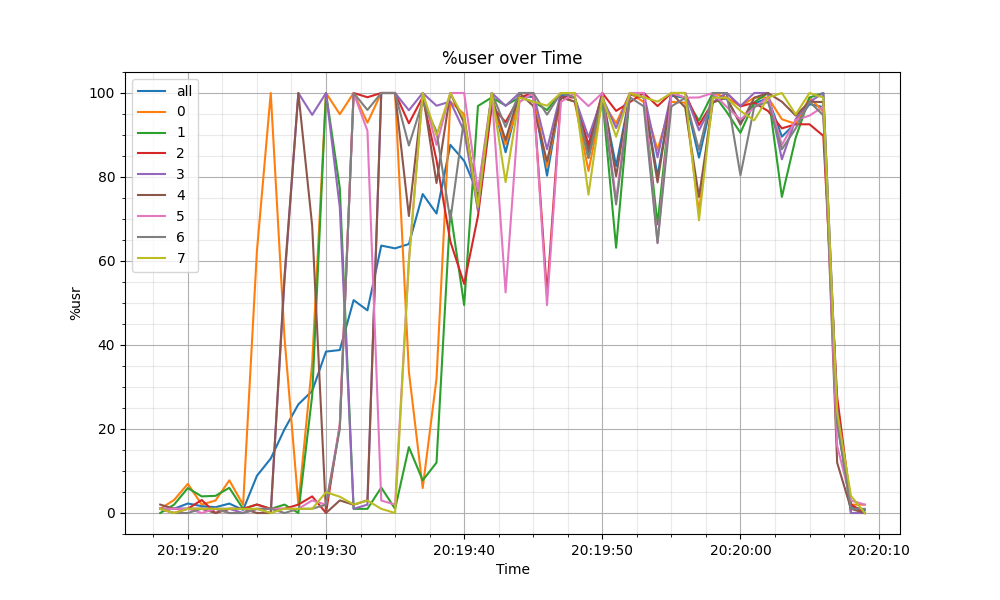
\includegraphics[width=\textwidth]{./cache/image/l1cache-usr-cpu.png}
Вот ещё есть график для idle\\
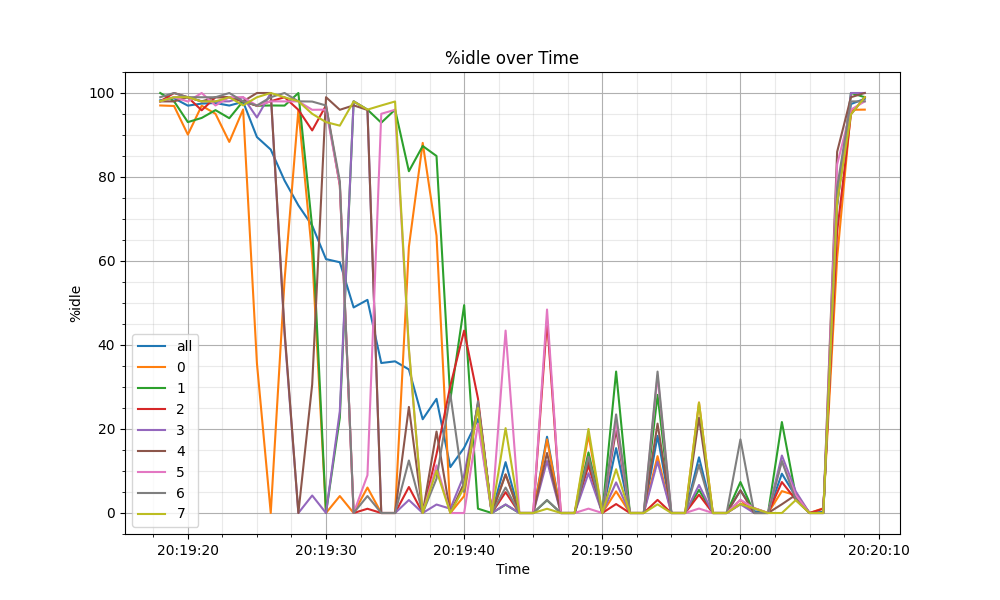
\includegraphics[width=\textwidth]{./cache/image/l1cache-idle-cpu.png}
Будем на них внимательно смотреть... шучу, сейчас будут более информативные графики.\\
\textbf{user time}\\
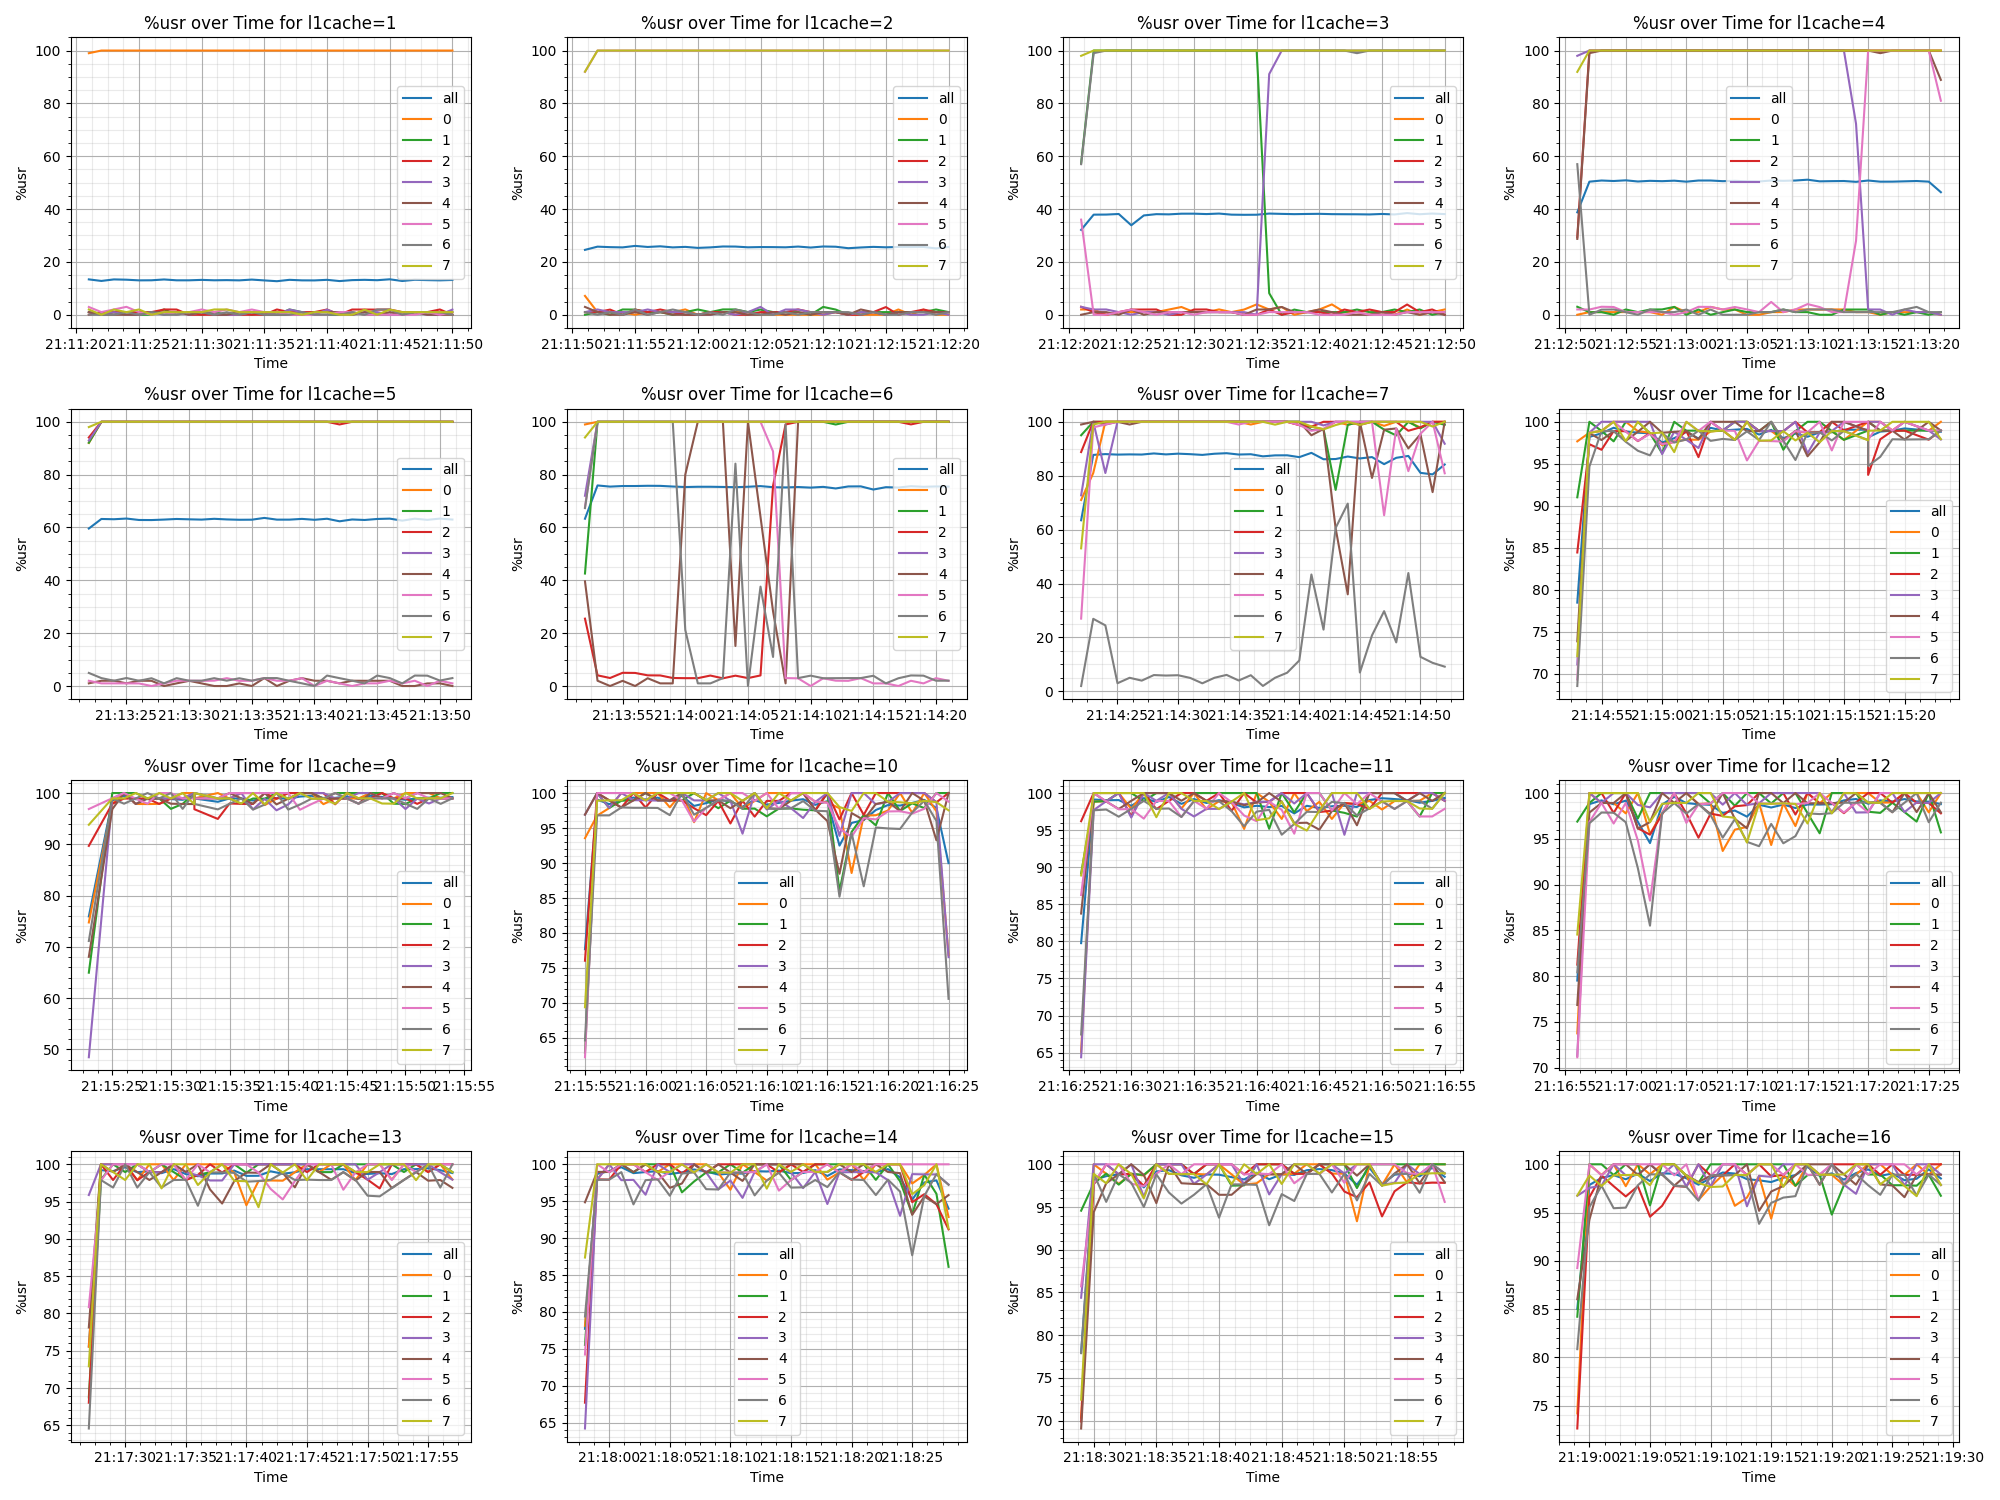
\includegraphics[width=\textwidth]{./cache/image/l1cache-each-usr-cpu.png}
\textbf{idle time}\\
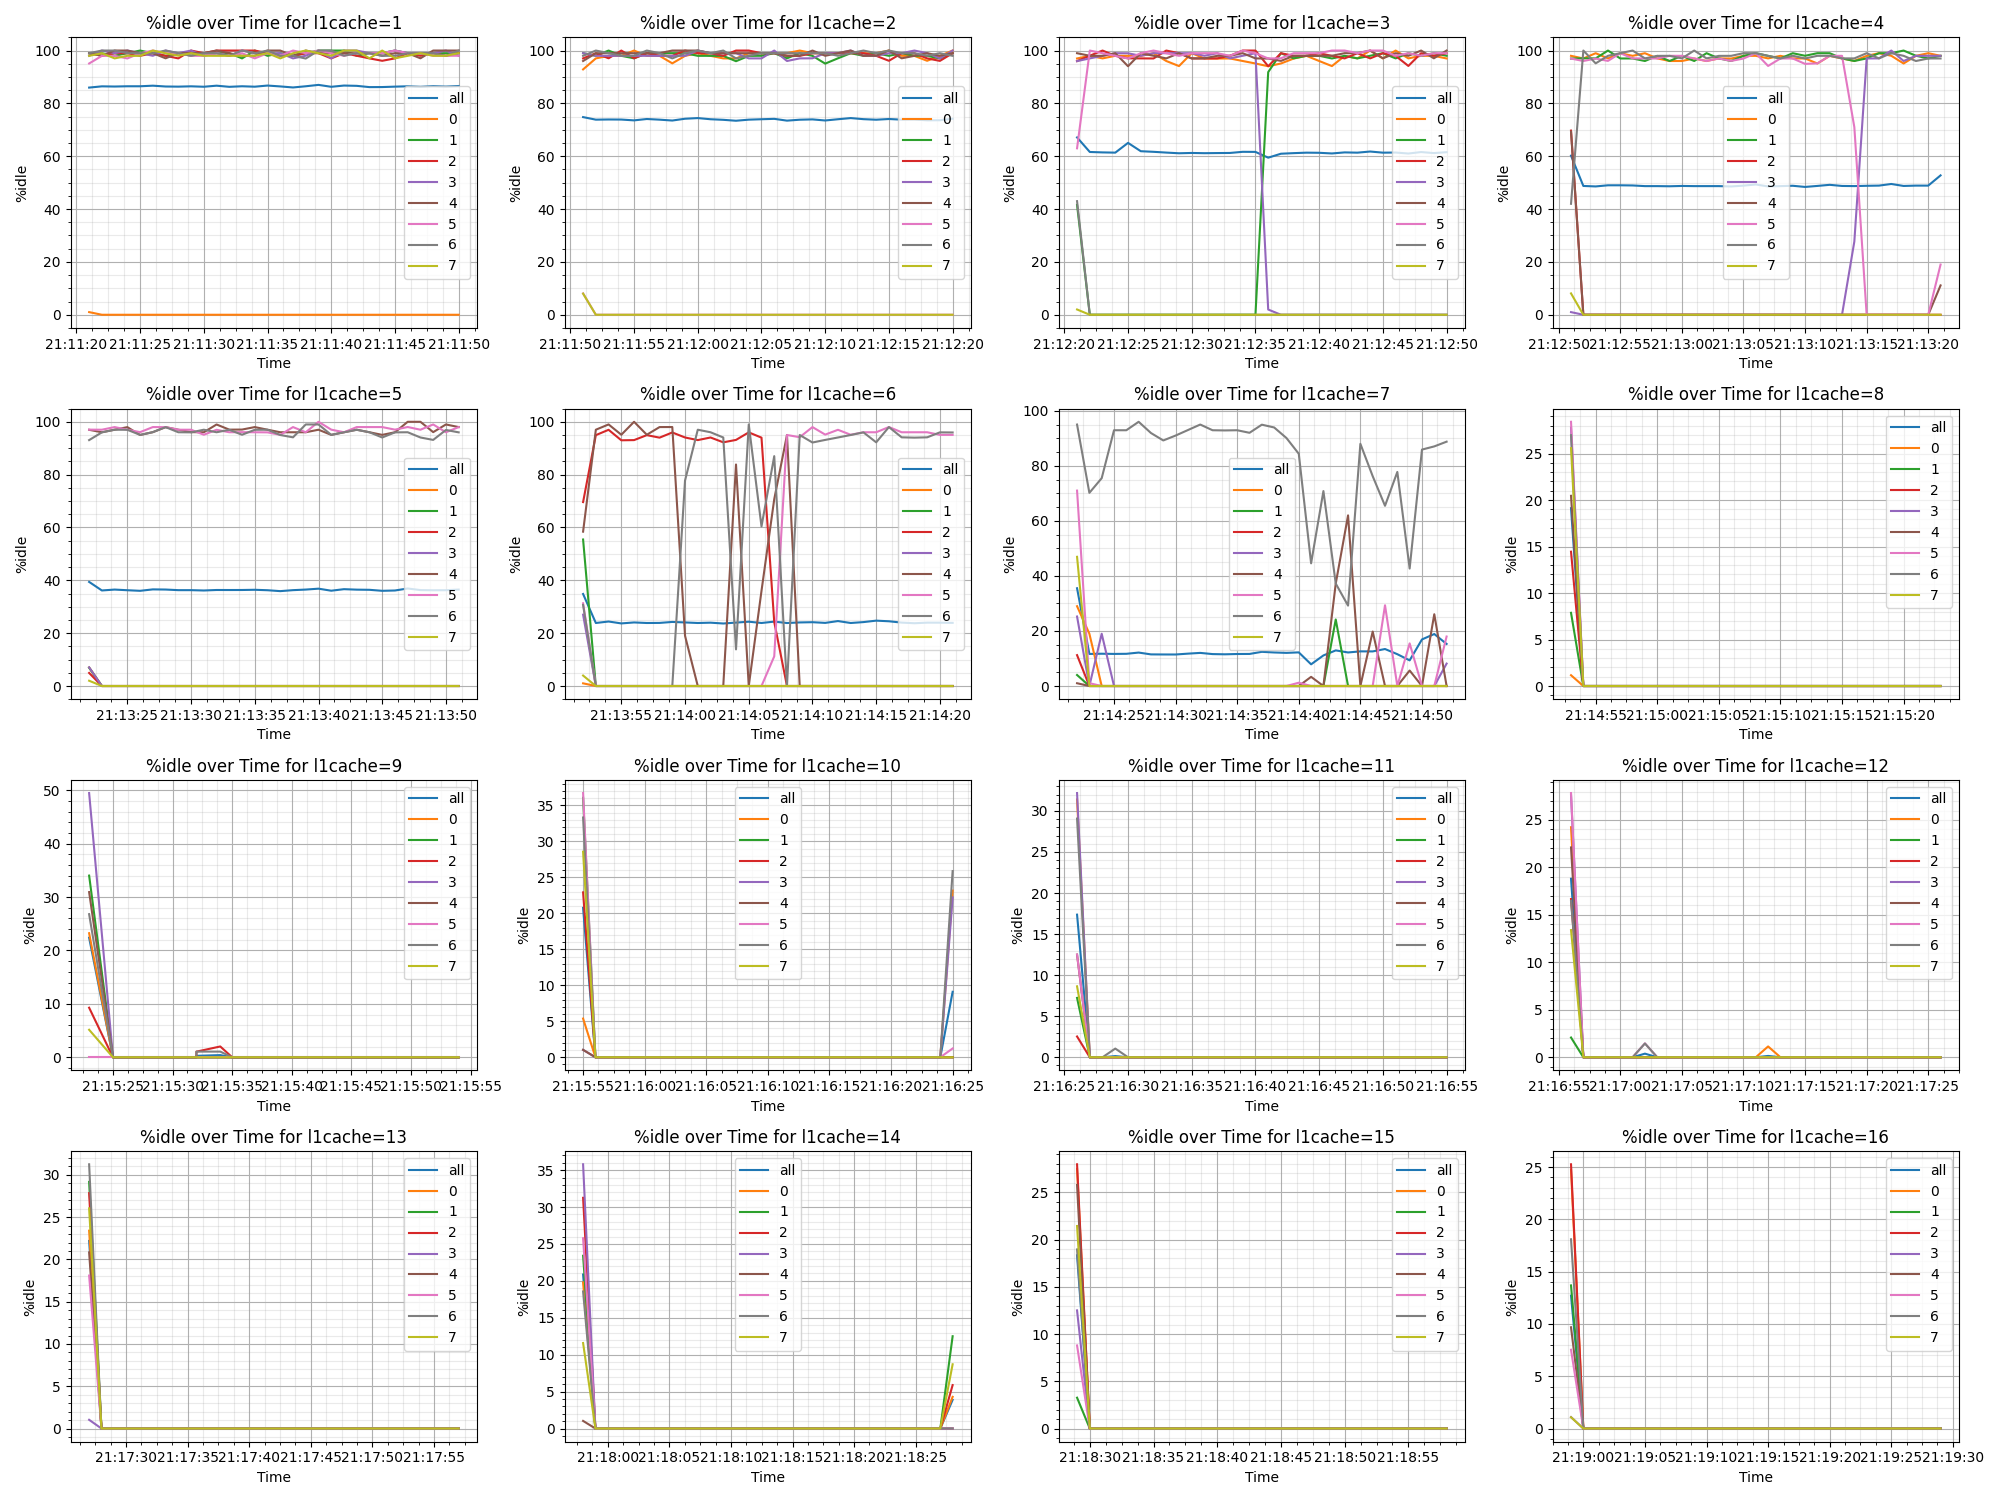
\includegraphics[width=\textwidth]{./cache/image/l1cache-each-idle-cpu.png}
Видим, что после 8 workers наши ядра заняты посностью, что соответсвует количеству виртуальных ядер на процессоре.\\
Так же из графиков видно, что если не все ядра заняты работой, то может произойти переключение на другое ядро из-за чего может упасть производительность.\\
Проверим наши доводы построив график \textit{bogo ops} от \textit{l1cache}.\\
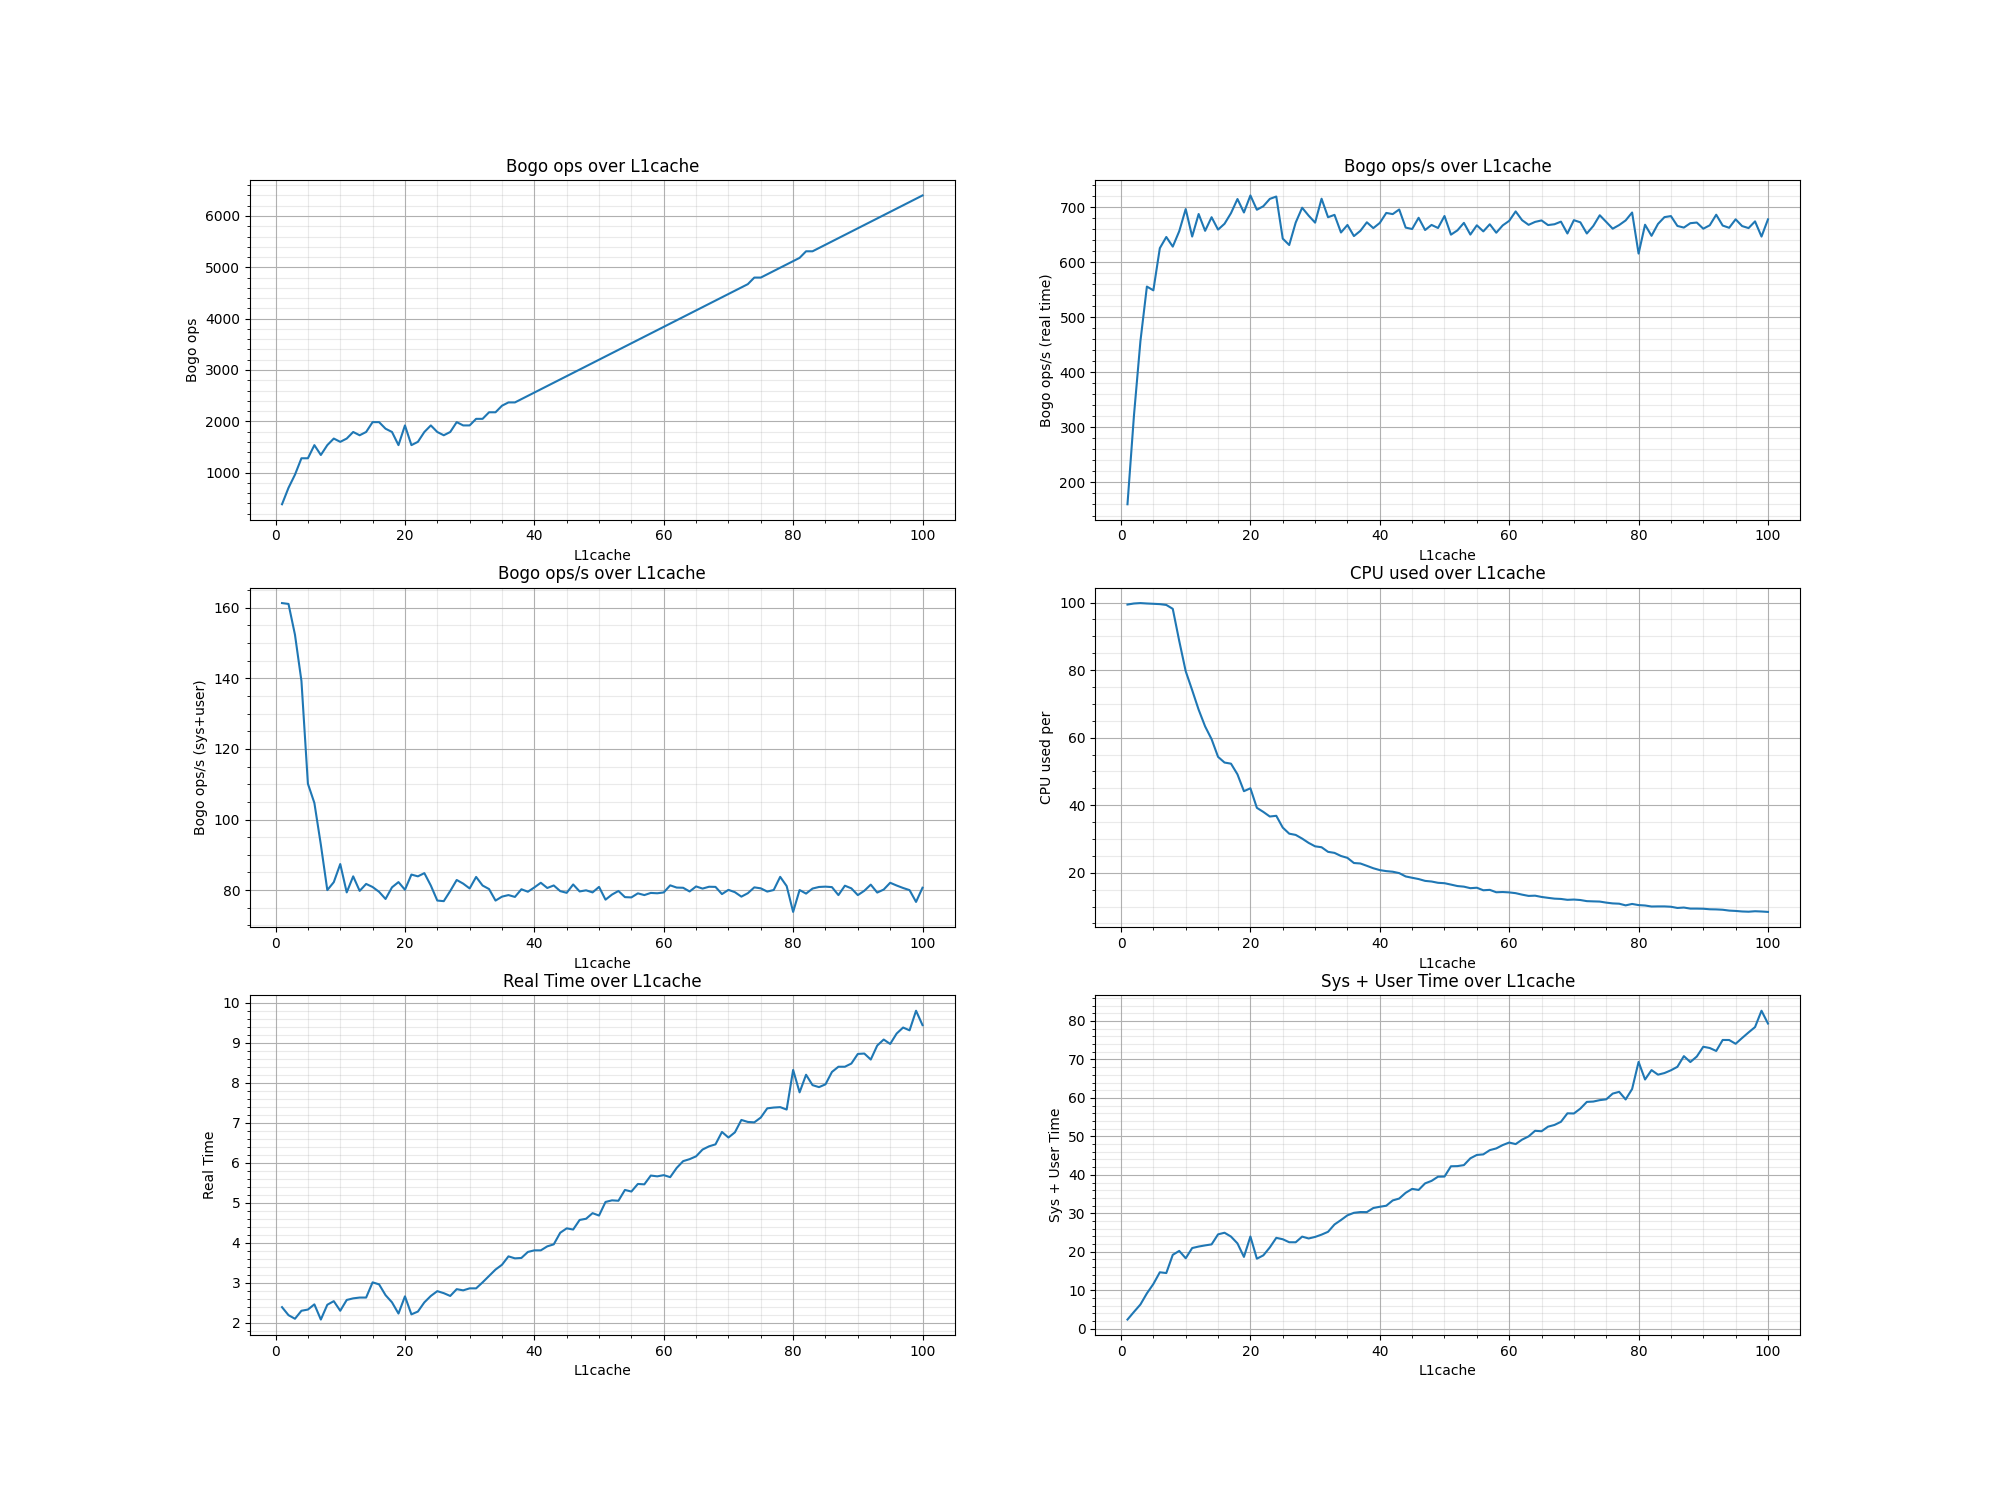
\includegraphics[width=\textwidth]{./cache/image/l1cache-bogops.png}
Видим, хоть с увеличением воркеров растет bogo ops, но нагрузка на каждый CPU (после 8 воркеров) падает. \\
Это увеличивает время ожидания в блокировке.\\
\textbf{Вывод:} оптимальное значение параметра l1cache равно 8.
\subsection{l1cache-sets}
Из документации stress-ng:
\nquote{--l1cache-sets N}{specify the number of level 1 cache sets}
Для нахождения оптималььного значения параметра l1cache-sets напишем простейший zsh-скрипт:
\VerbatimInput{./cache/scripts/l1cache-sets-testing.zsh}
\VerbatimInput{./cache/scripts/l1cache-sets.txt}
\textbf{Графики...графики...графики...}\\
\textbf{user time}\\
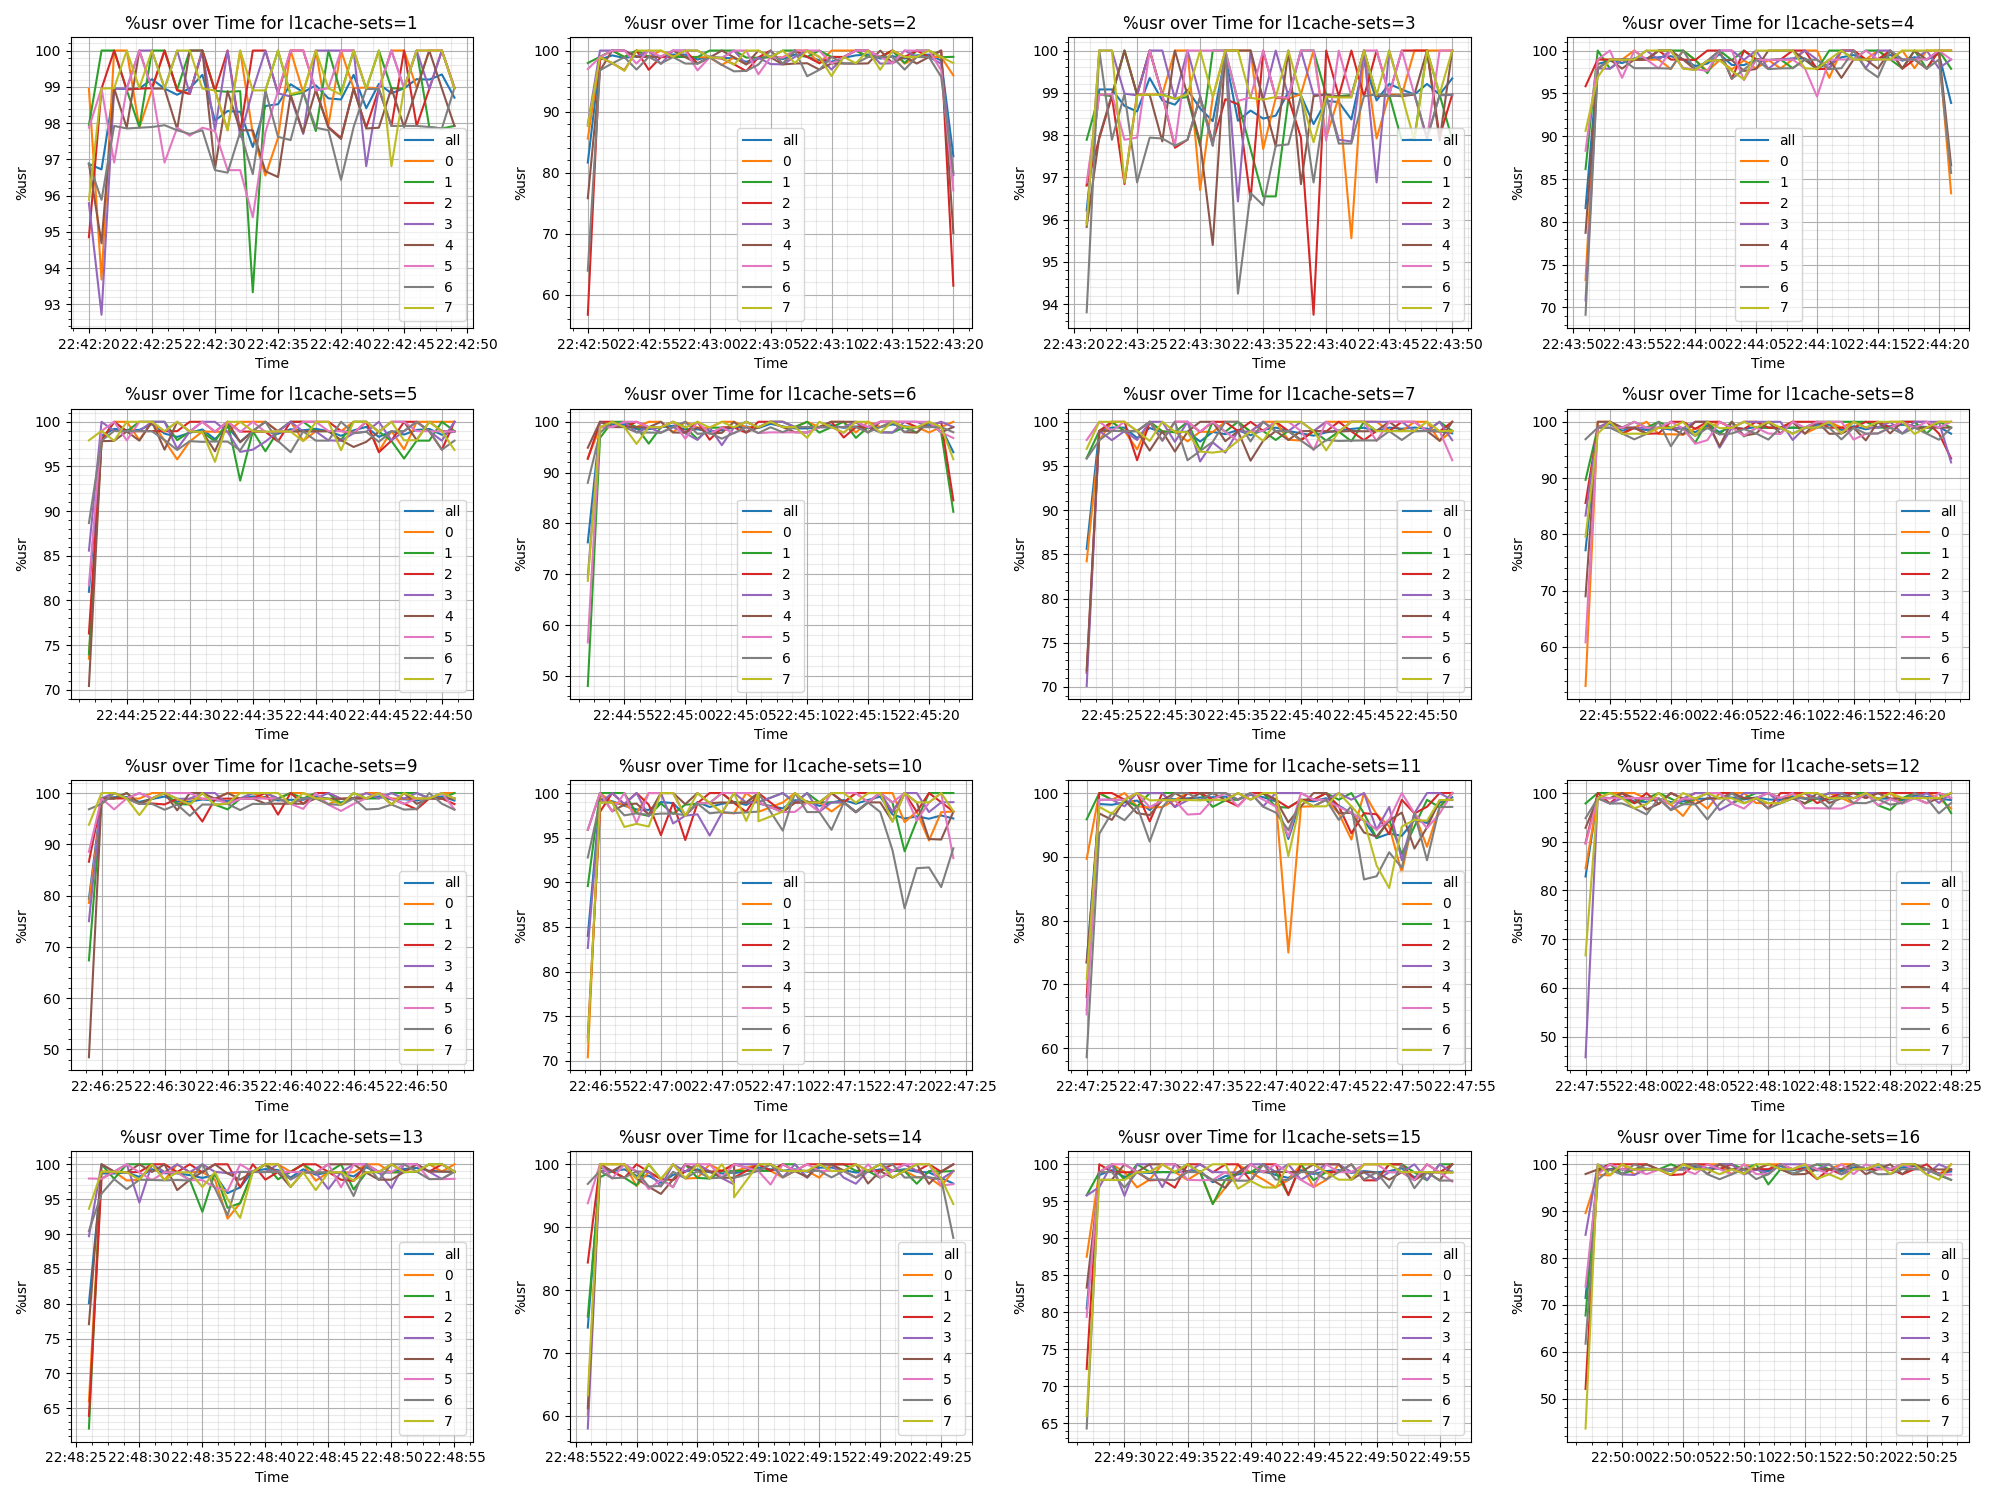
\includegraphics[width=\textwidth]{./cache/image/l1cache-sets-usr-cpu.png}
\textbf{idle time}\\
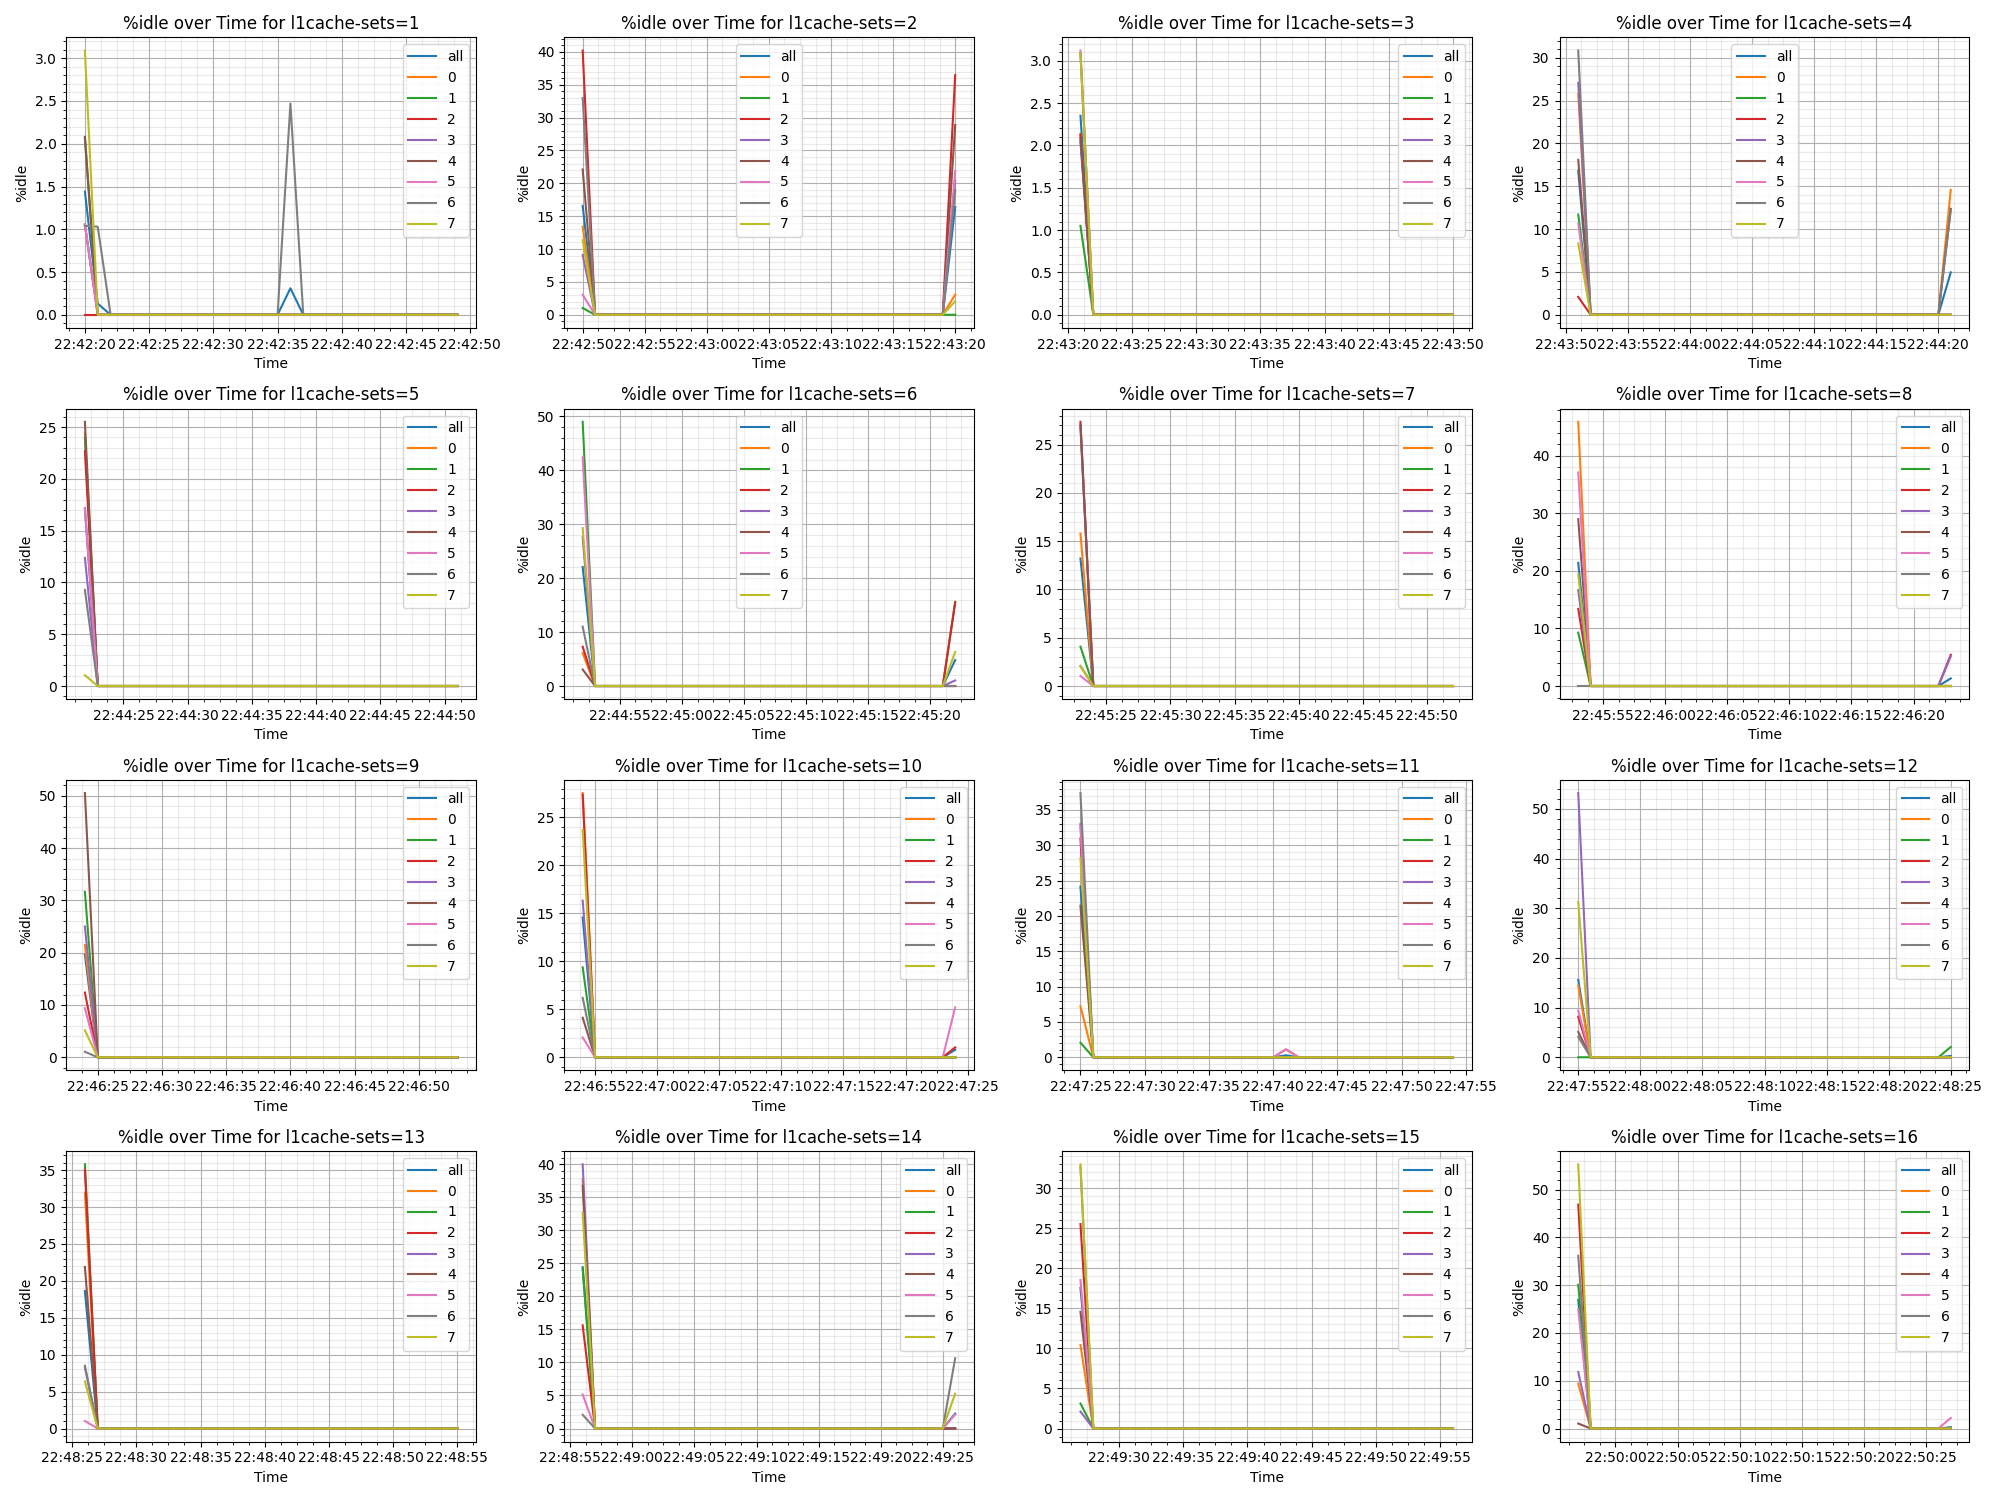
\includegraphics[width=\textwidth]{./cache/image/l1cache-sets-idle-cpu.png}
\textbf{sys time}\\
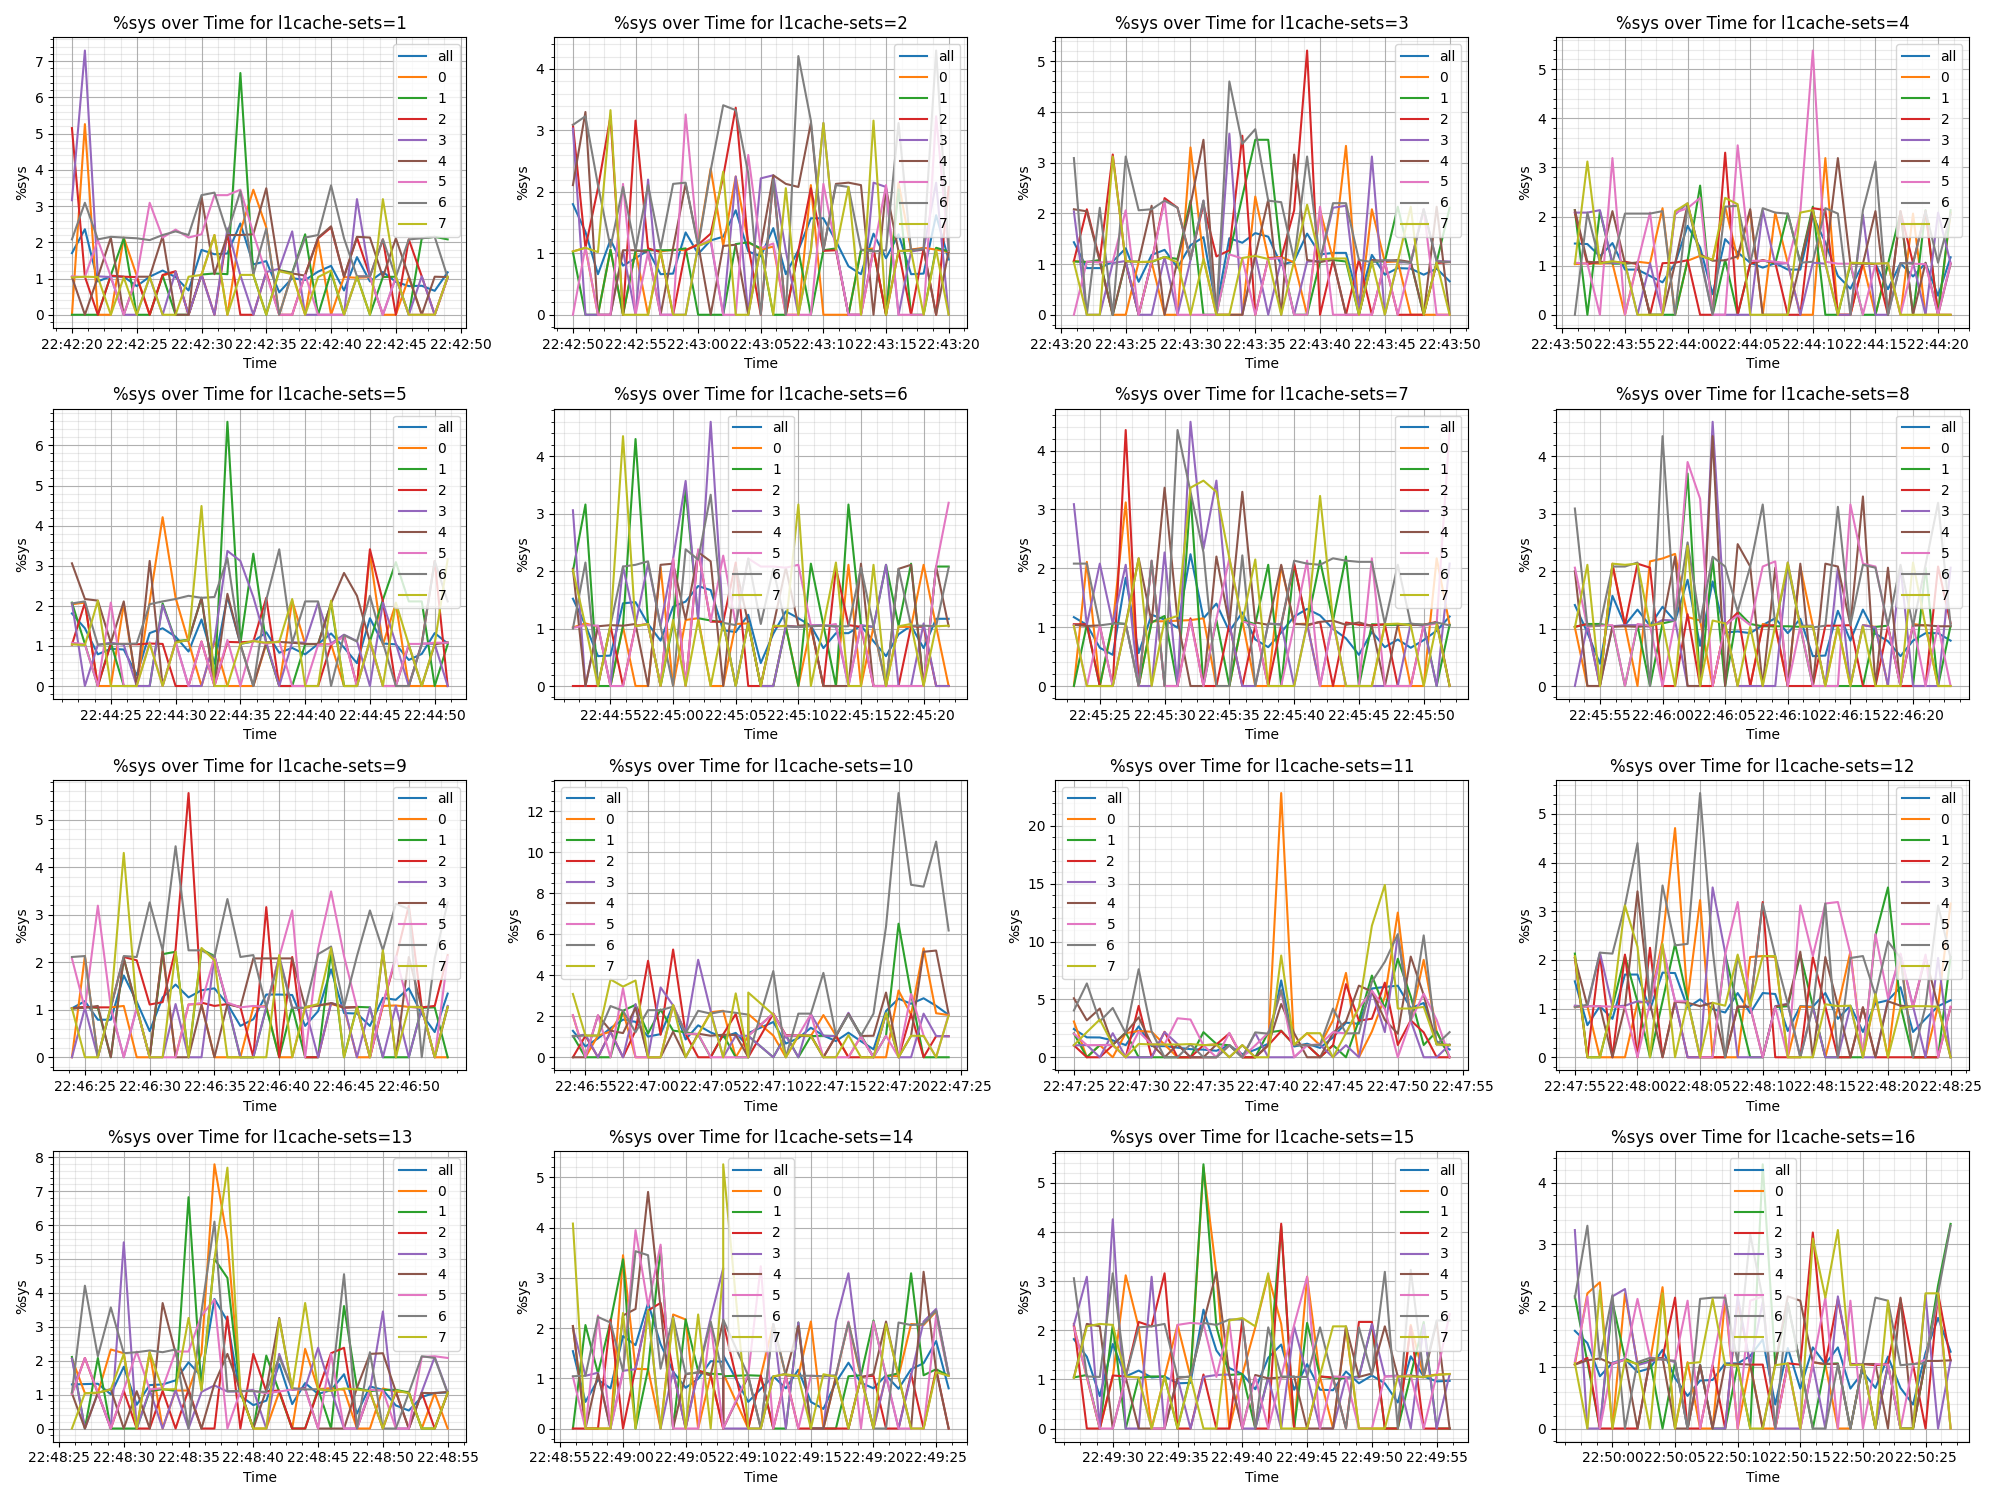
\includegraphics[width=\textwidth]{./cache/image/l1cache-sets-sys-cpu.png}
Делаем вывод что чем больше set, тем выше bogo-ops.\\
Тут должен быть \textit{perf}, но у меня он ничего не поддерживает:\\
\begin{verbatim}
sudo perf stat -B -e cache-references,cache-misses,cycles,instructions,branches,faults,migrations,L1-dcache-loads,L1-dcache-load-misses,L1-dcache-stores stress-ng --l1cache 8 --l1cache-sets 8 --metrics --timeout 30
stress-ng: info:  [161315] setting to a 30 second run per stressor
stress-ng: info:  [161315] dispatching hogs: 8 l1cache
stress-ng: info:  [161316] stress-ng-l1cache: l1cache: size: 32.0K, sets: 8, ways: 8, line size: 64
stress-ng: info:  [161315] successful run completed in 30.63s
stress-ng: info:  [161315] stressor       bogo ops real time  usr time  sys time   bogo ops/s     bogo ops/s CPU used per
stress-ng: info:  [161315]                           (secs)    (secs)    (secs)   (real time) (usr+sys time) instance (%)
stress-ng: info:  [161315] l1cache            2264     30.47    238.64      1.11        74.30           9.44        98.35

    Performance counter stats for 'stress-ng --l1cache 8 --l1cache-sets 8 --metrics --timeout 30':

    <not supported>      cache-references                                                      
    <not supported>      cache-misses                                                          
    <not supported>      cycles                                                                
    <not supported>      instructions                                                          
    <not supported>      branches                                                              
                1678      faults                                                                
                    9      migrations                                                            
    <not supported>      L1-dcache-loads                                                       
    <not supported>      L1-dcache-load-misses                                                 
    <not supported>      L1-dcache-stores                                                      

        30,642159810 seconds time elapsed

        238,688613000 seconds user
        1,177890000 seconds sys
\end{verbatim}

Попробуем провести тот же тест но с большими set
\VerbatimInput{./cache/scripts/l1cache-sets-testing-2.zsh}
\VerbatimInput{./cache/scripts/l1cache-sets-testing-2.txt}
\textbf{Графики...графики...графики...}\\
\textbf{user time}\\
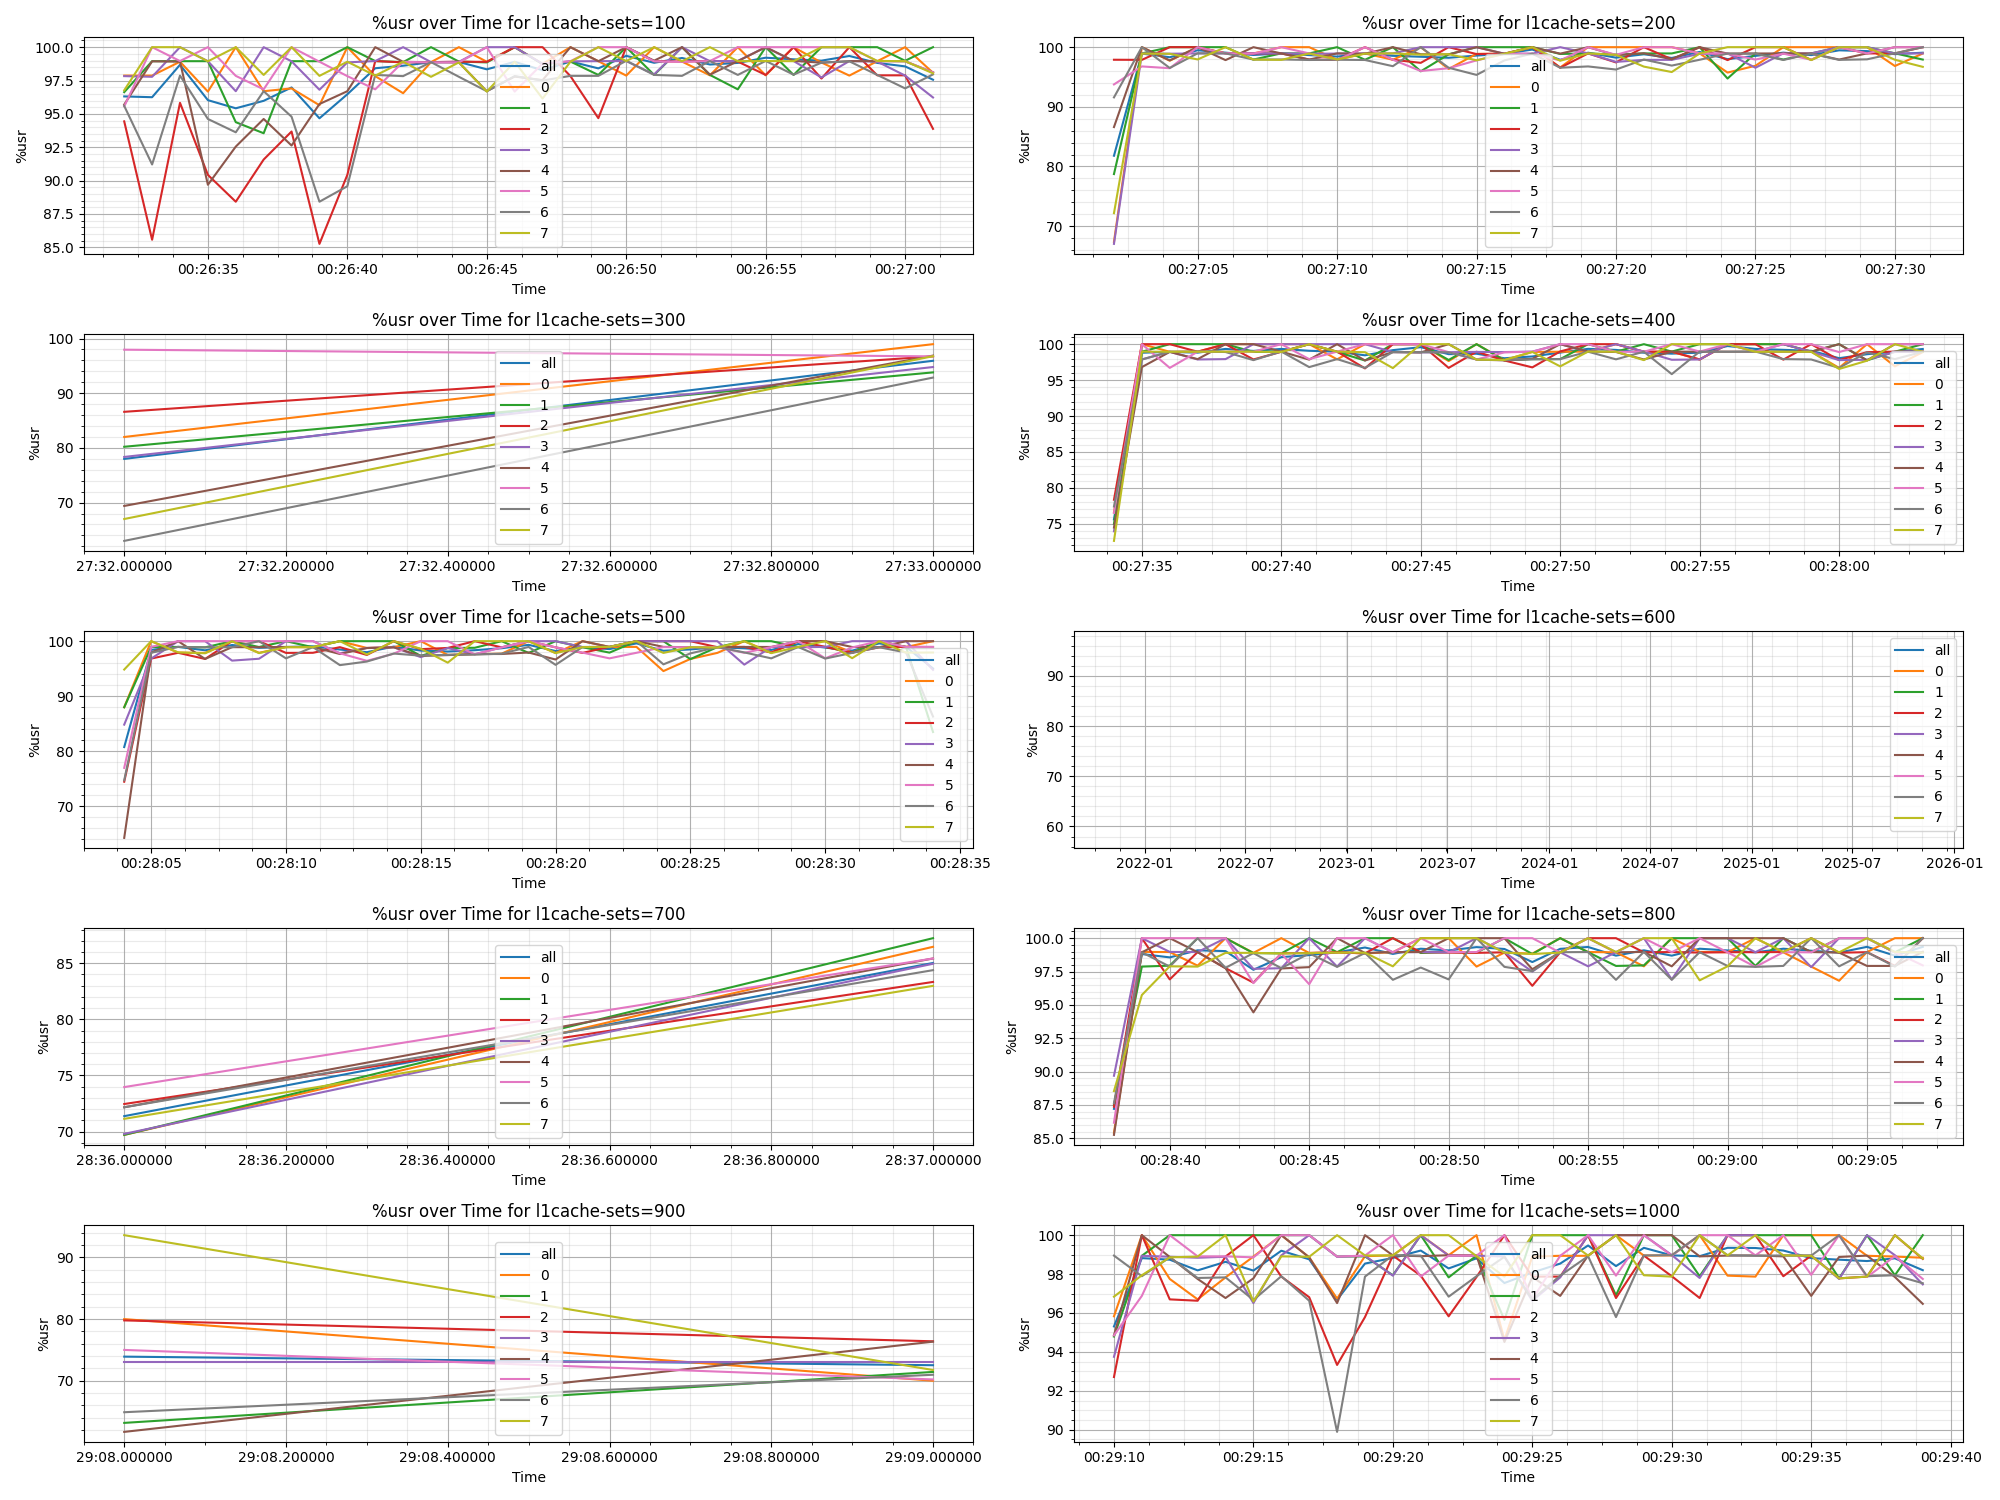
\includegraphics[width=\textwidth]{./cache/image/l1cache-sets-usr-cpu-2.png}
\textbf{idle time}\\
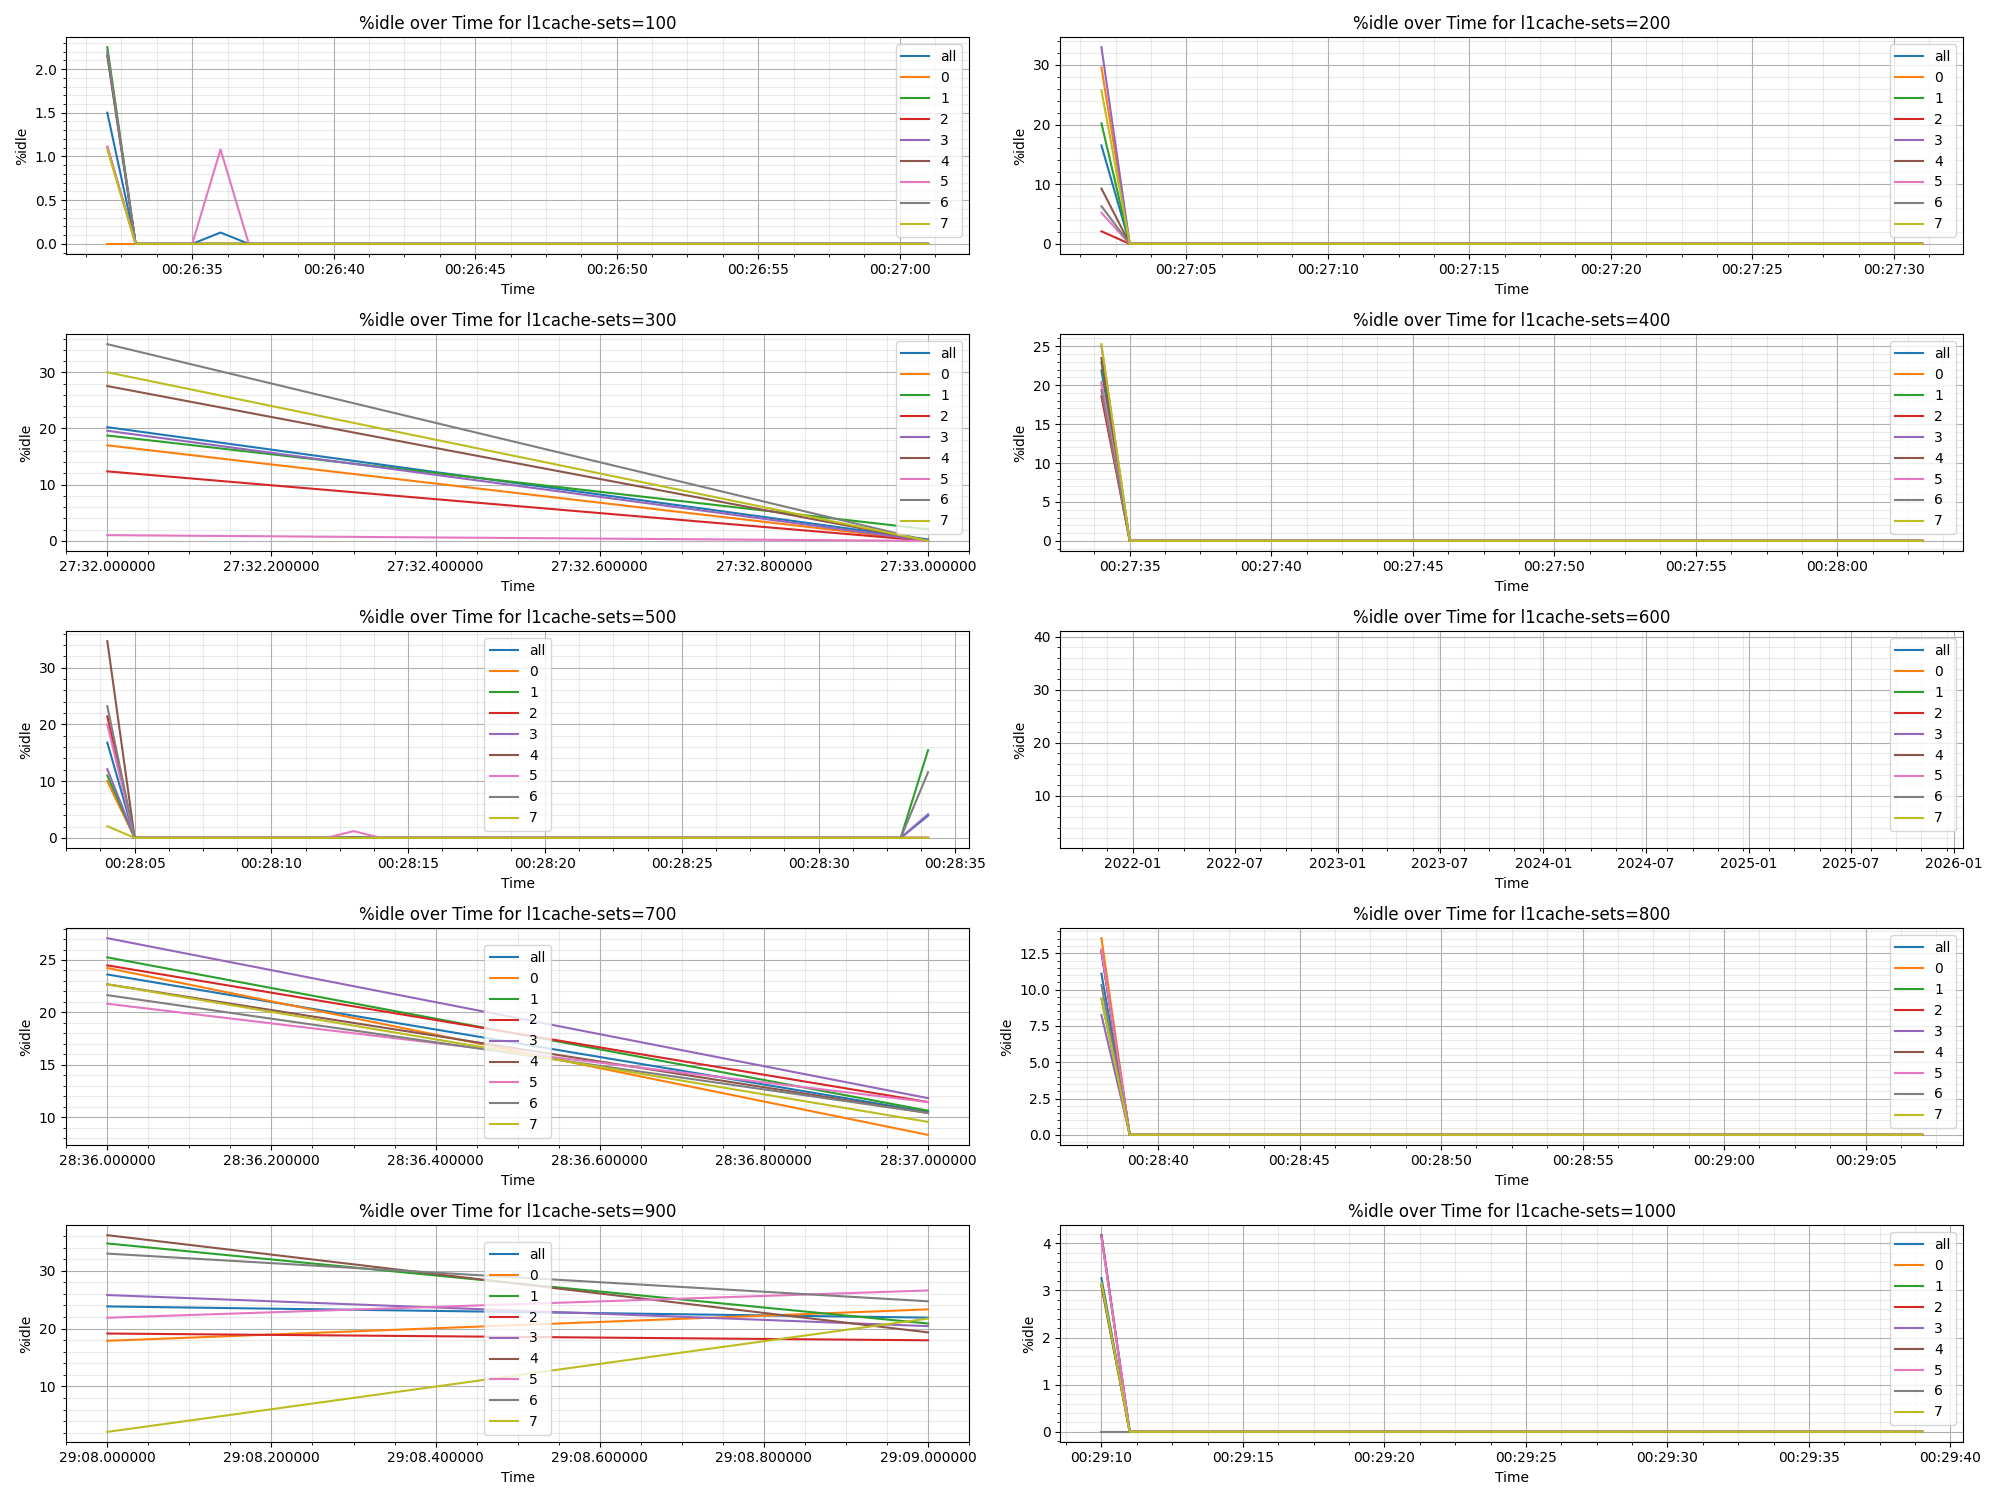
\includegraphics[width=\textwidth]{./cache/image/l1cache-sets-idle-cpu-2.png}
\textbf{sys time}\\
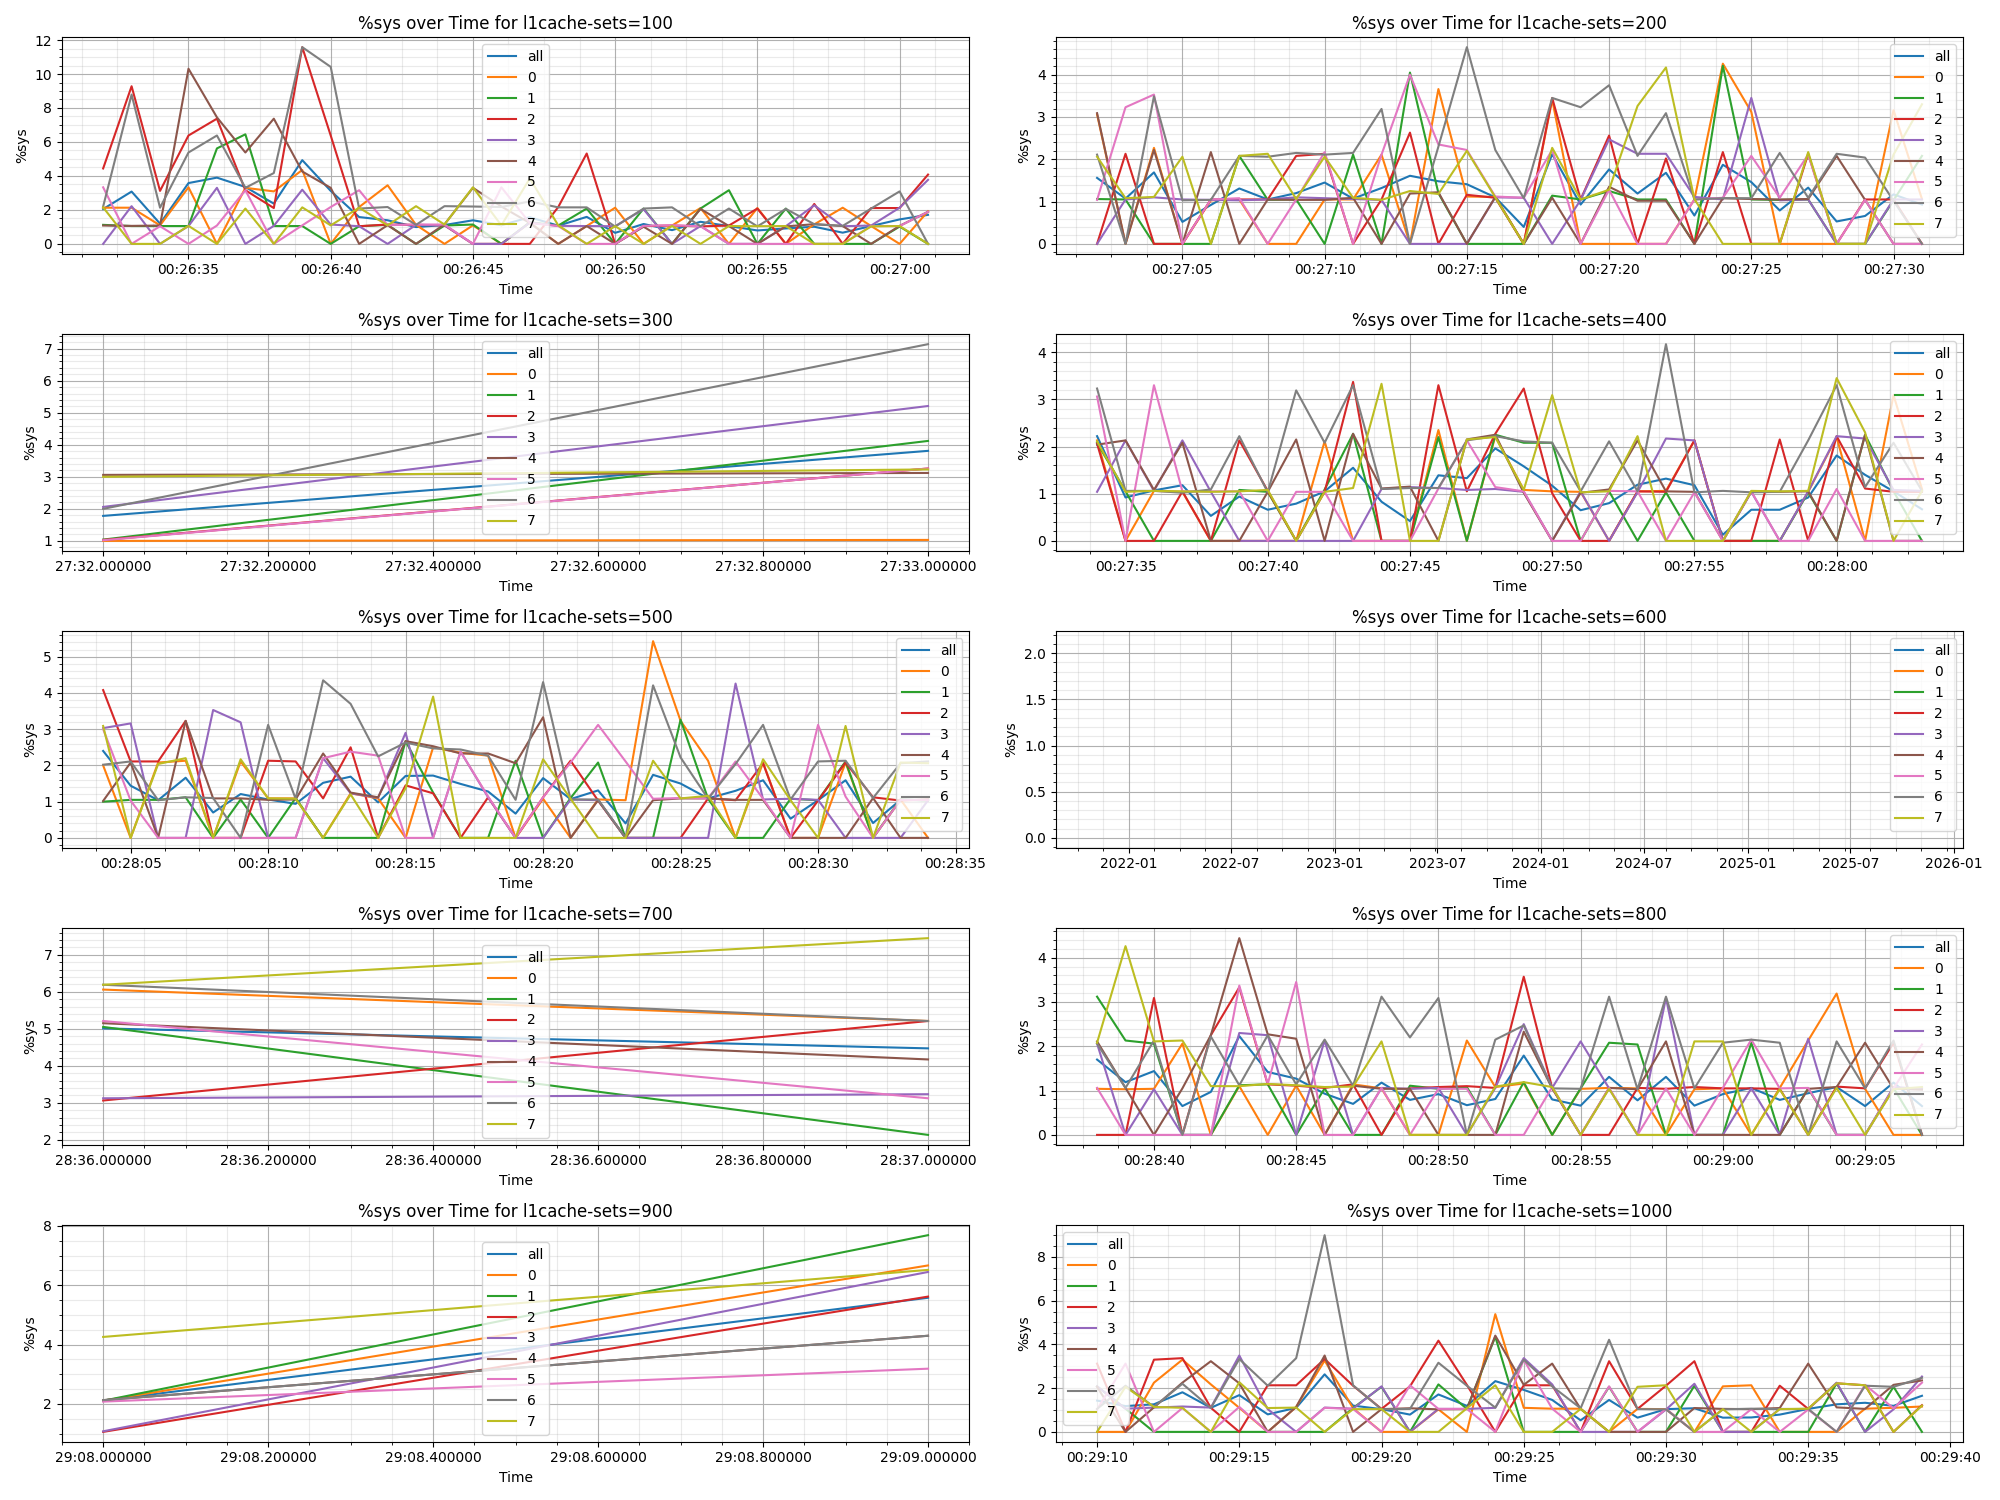
\includegraphics[width=\textwidth]{./cache/image/l1cache-sets-sys-cpu-2.png}
\textbf{Вывод:} чем больше set, тем выше bogo-ops, но при этом увеличивыется вероятность того, что тест сломается. (приведена лучшая попытка)\\
Еще посмотрим графики \textit{bogo ops}, чтобы проверить наш вывод\\
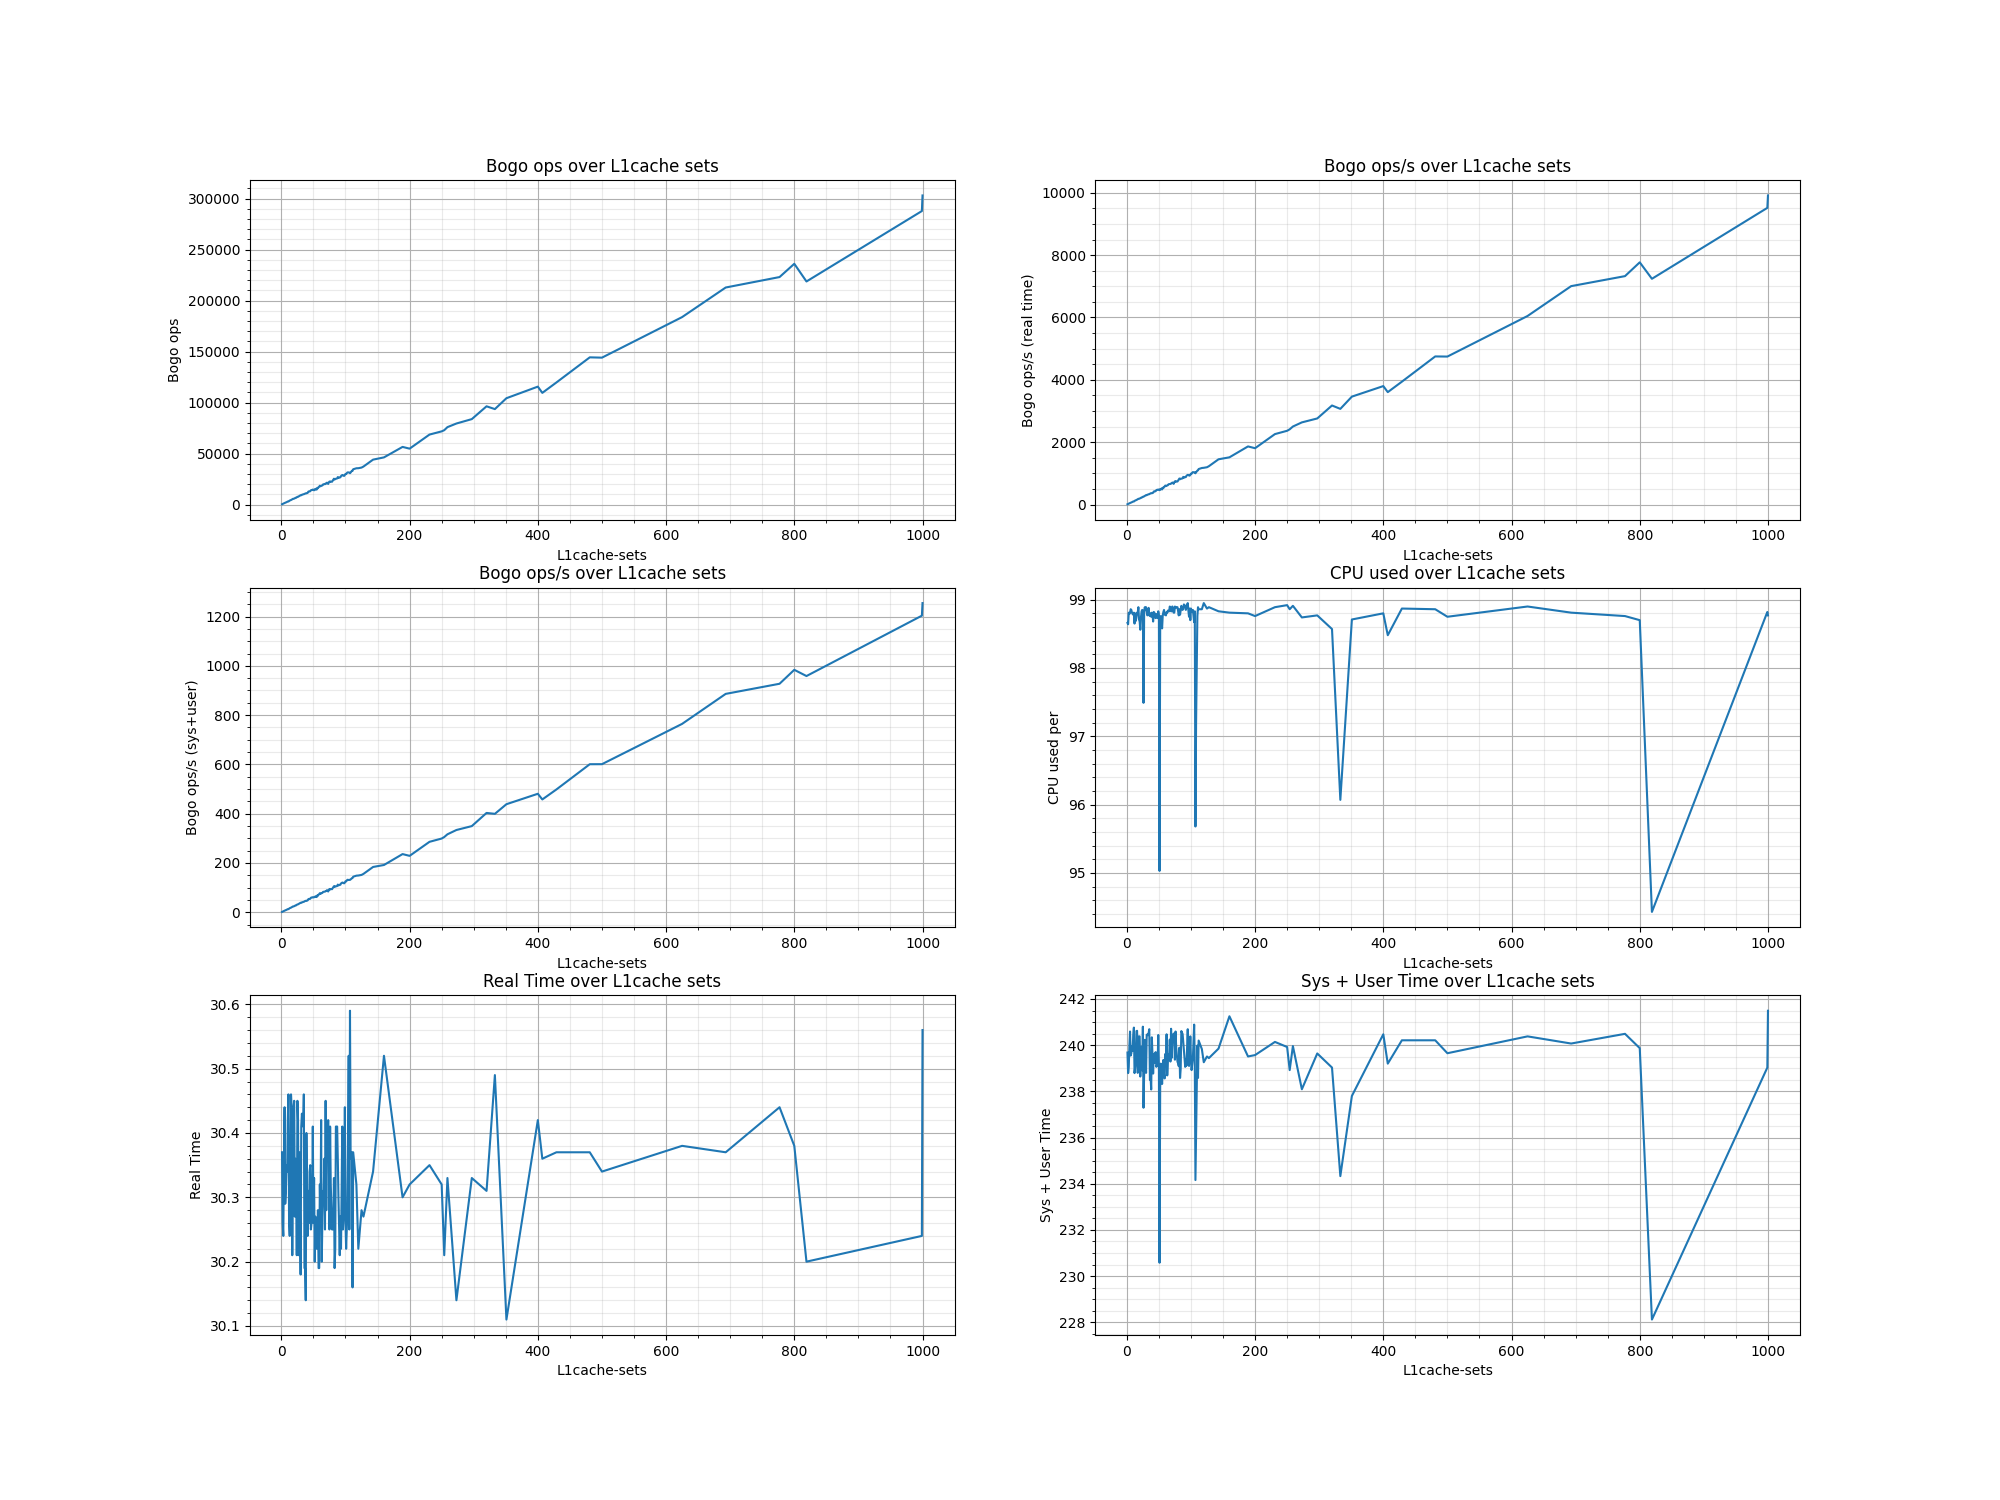
\includegraphics[width=\textwidth]{./cache/image/l1cache-sets-bogops.png}
Видим, что вывод оказался верным, что чем больше set, тем выше bogo-ops, но при этом увеличивыется вероятность того, что тест сломается.
\subsection{cache-fence}
Из документации stress-ng:
\nquote{--cache-fence}{force  write  serialization on each store operation (x86 only). This is a no-op for non-
x86 architectures.}
\VerbatimInput{./cache/scripts/l1cache-fence.zsh}
\VerbatimInput{./cache/scripts/l1cache-fence.txt}
\textbf{Графики...жирафики}\\
\textbf{user time}\\
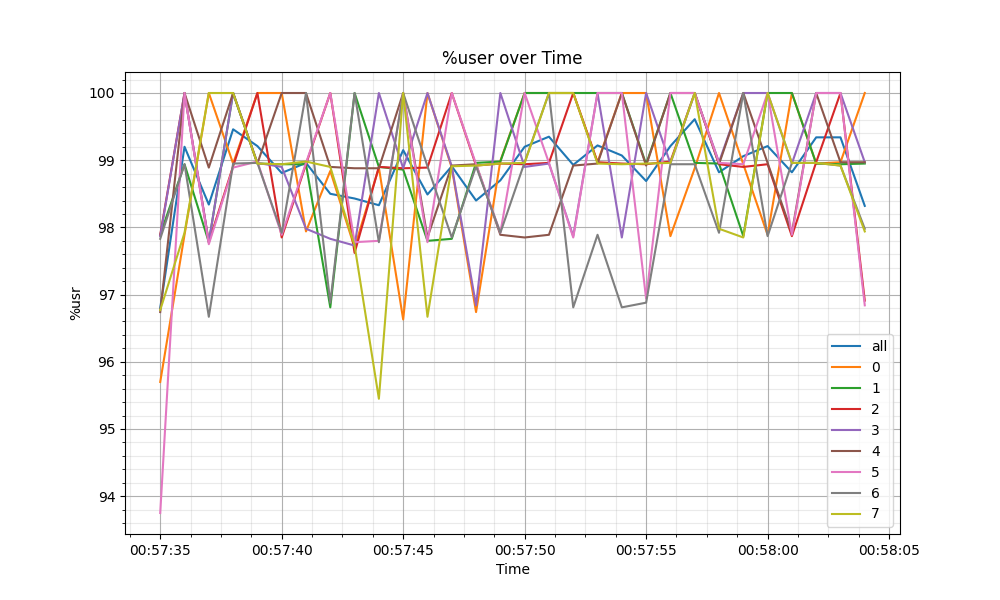
\includegraphics[width=\textwidth]{./cache/image/l1cache-fence-usr.png}
\textbf{idle time}\\
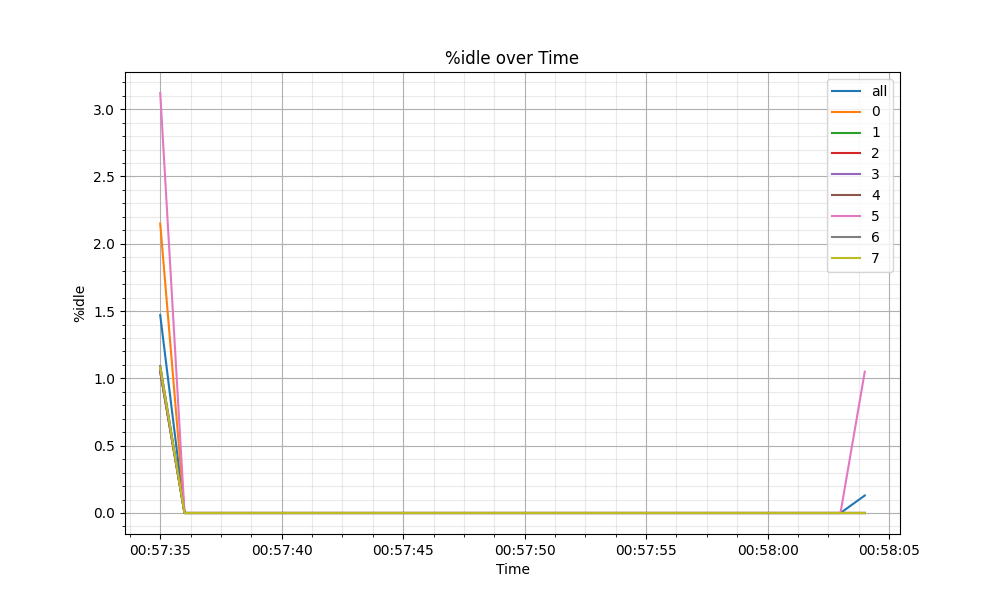
\includegraphics[width=\textwidth]{./cache/image/l1cache-fence-idle.png}
\textbf{sys time}\\
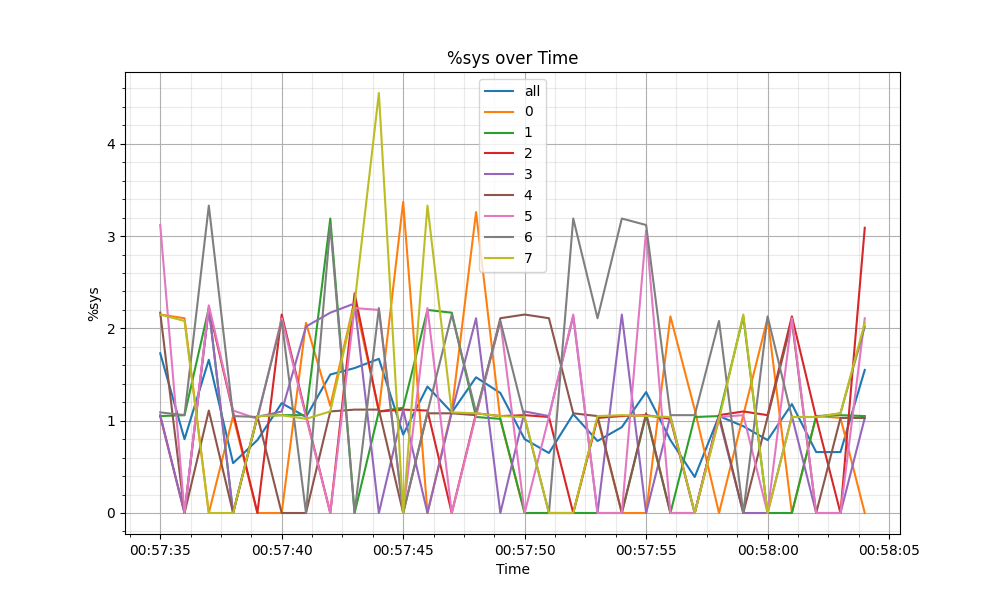
\includegraphics[width=\textwidth]{./cache/image/l1cache-fence-sys.png}
\textbf{Вывод:} --cache-fence дает нам небольшой выигрыш по производильности.\\

